In this example, we run through the requirements that are necessary for
simulation (fitting) of EXAFS data relevant to a sample experiment obtain signal
from a \SI{5}{\micro\metre} thick Fe foil. The simulation will be carried out for
ambient conditions Fe foil; a future enhancement of SIMEX will take P-T
conditions from hydrocode simulations before performing high-pressure
XANES/EXAFS calculations.

To validate the EXAFS simulations, we compare the simulated spectrum with raw
data obtained from an X-ray absorption beamline at the ESRF synchrotron. The
normalized XAS spectrum for a \SI{5}{\micro\metre} thick Fe foil is shown in figure 1.
\begin{figure}
  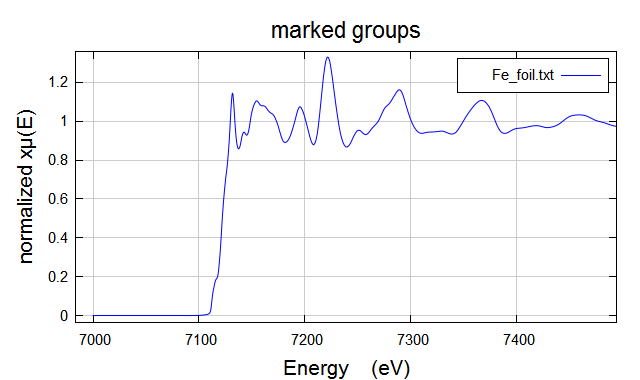
\includegraphics[width=4.822in,height=2.528in]{figures/Task42210-img001.png}
  \caption{%
    X-ray absorption spectra collected at BM23 (EXAFS beamline, ESRF) of
    a \SI{5}{\micro\metre} thick iron foil.%
  }
  \label{fig:xafs_fig1}
\end{figure}
Calculations of XAFS spectra are performed using the FEFF package. FEFF uses a
single input file to select which modules should be run inside the program and
what parameters should be used. The material of interest is contained within
this input file based on its crystallographic parameters and atomic positions.
The ATHENA program is able to combine crystallographic input files (.cif format)
for a chosen material into the FEFF .inp format. The .cif files can typically be
found from most crystallographic database websites or can be manually created
using gui programs such as VESTA. FEFF is then run to calculate the paths
between atoms and is then saved / exported for use by other third party programs
(such as ARTEMIS) to compare with actual data.

\subsection{Artemis User Guide} A more comprehensive user guide for running ARTEMIS
/ FEFF can be found at
\href{http://bruceravel.github.io/demeter/artug/index.html}{http://bruceravel.github.io/demeter/artug/index.html}.

\begin{figure}
  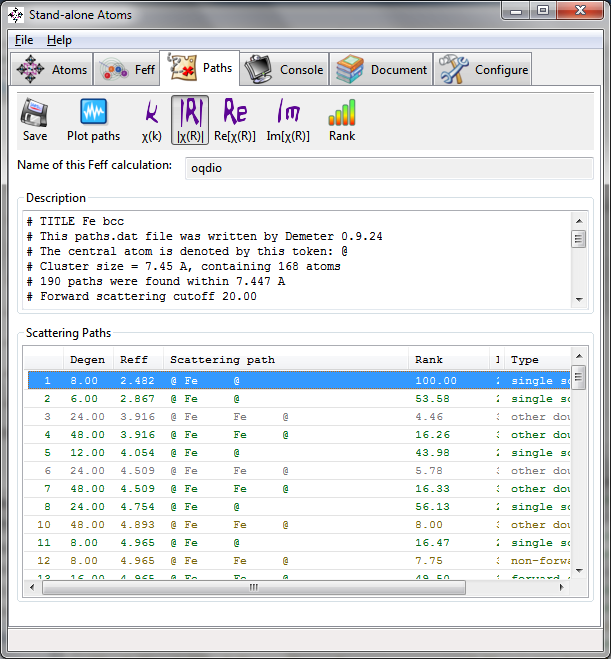
\includegraphics[width=4.3063in,height=4.6465in]{figures/Task42210-img002.png}
  \caption{%
    Screenshot of the output data collected in the ATOMS software after
    running Feff simulation of Fe at ambient conditions.
  }
  \label{fig:xafs_fig2}
\end{figure}

\begin{figure}
  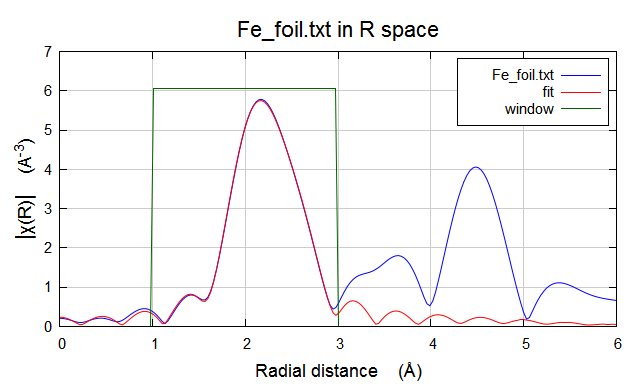
\includegraphics[width=4.852in,height=2.9173in]{figures/Task42210-img003.png}
  \caption{%
    Fitting of the first Fe shell from FEFF calculations (red) to Fe EXAFS
    data collected on BM23 beamline, ESRF (blue)
  }
  \label{fig:xafs_fig3}
\end{figure}

\subsection{Simulating XANES at shock conditions}
Shock compression experiments on Fe have previously been carried out at the ESRF
\cite{Torchio2016}. In that study,
simulations of the XANES at shock conditions were carried out using the ABINIT
code and are shown below in figure 4.

\begin{figure}
  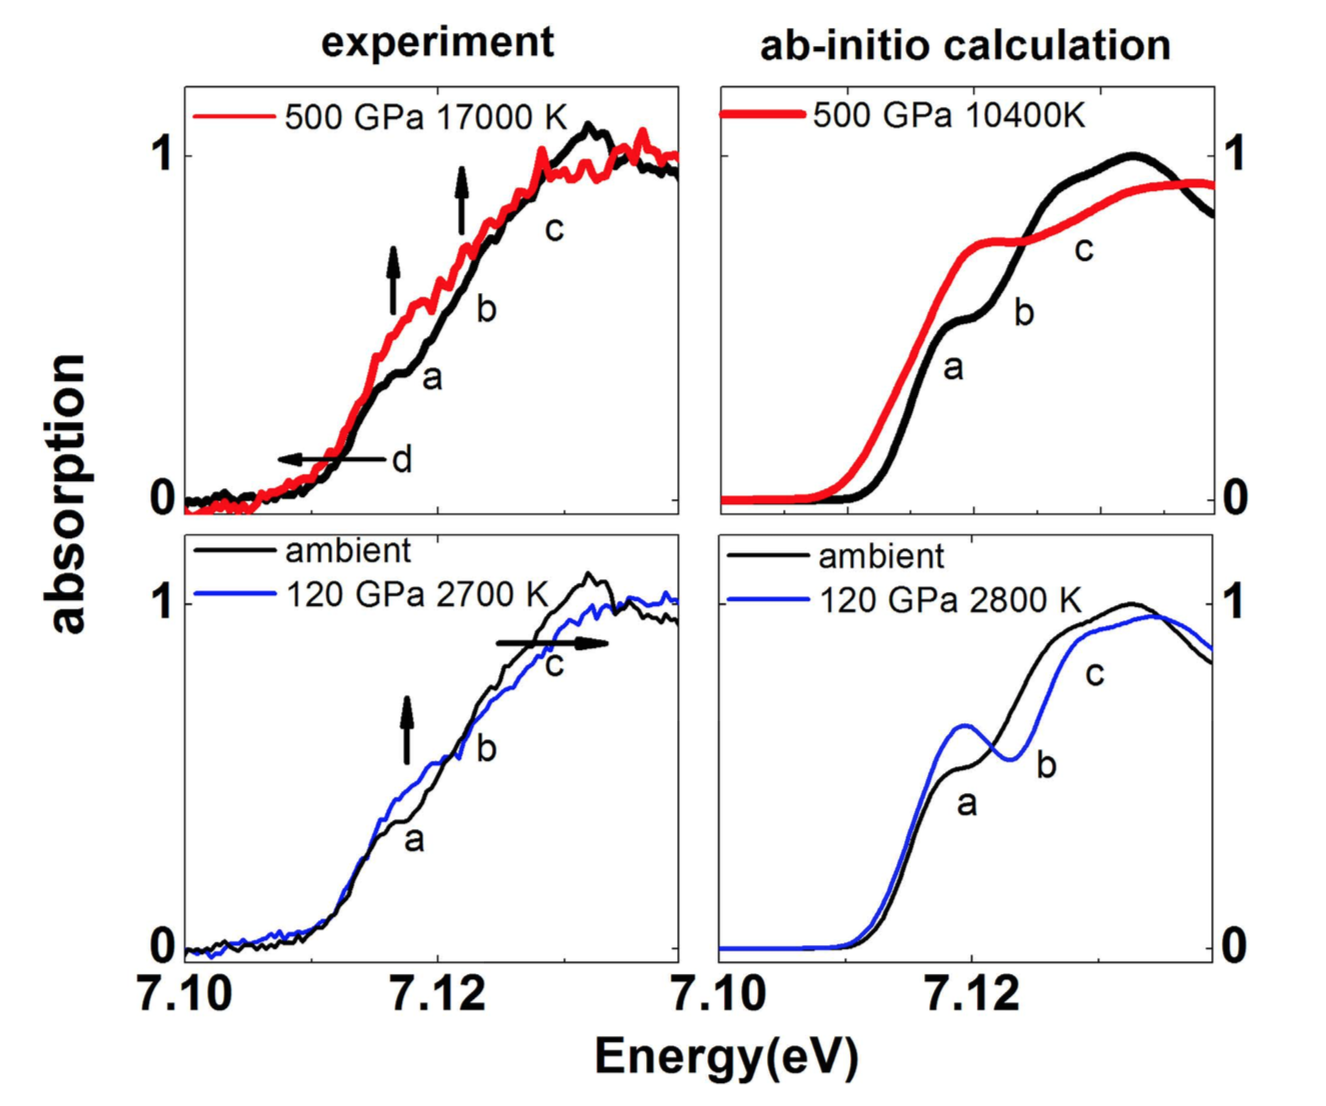
\includegraphics[width=4.3063in,height=3.5945in]{figures/Task42210-img004.png}
  \caption{%
    Comparisons of the absorption edge of Fe between experiments (left
    panels) and ab-initio calculations (right panels) at
    \SIlist{120;150}{\giga\pascal}. Figure
  taken from Ref.~\cite{Torchio2016}.
  }
  \label{fig:xafs_fig4}
\end{figure}
